
\subsection{Lunghezza di attenuazione}

La possibilità di fare misure locali con il miniscint 
\marginpar{dobbiamo chiamarlo miniscint?}
ci permette di misurare la lunghezza di attenuazione del sistema scintillatore più guida di luce. Avendo preso misure soltanto sullo scintillatore potrebbe sembrare che abbiamo misurato soltanto la sua lunghezza di attenuazione, ma la nostra strumentazione rivela un evento soltanto quando i fotoni rilasciati raggiungono il PMT dopo aver attraversato la guida di luce. 
Abbiamo eseguito le misure dividendo il PM1 in 16 caselle e ponendo su ognuna di esse il miniscint nei punti mostrati in \emph{figura}. 
\marginpar{inserire disegno, descrizione e dimensioni miniscint}

Nel fare le misure sulle caselle periferiche abbiamo appoggiato il miniscint sulla struttura che circonda il PM1 in modo che l'angolo tra esso ed il miniscint sia sempre lo stesso. Tale accorgimento ci permette di usare quelle misure per stimare l'efficienza locale (relativa) del PM1 \emph{che sarà trattata in dettaglio in una delle sezioni seguenti  (dire quale) }.                            \marginpar{spiegare quel ``relativa'' nella relazione completa}
Per ogni casella abbiamo acquisito il numero di coincidenze verificatesi in \SI{1000}{s}. Al PM1 era collegata l'ADC in modo da poter registrare anche il rilascio di energia in ogni sezione.

Se chiamiamo $N$ il numero di muoni che attraversano ogni casella, possiamo legare questa quantità alla lunghezza di attenuazione attraverso la relazione \eqref{exp} in cui $x$ è la distanza orizzontale del miniscint dalla guida di luce; $N_0$ e $\lambda$ sono i parametri del fit. 
\begin{equation}
N=N_0 e^{-\frac{x}{\lambda}}  \label{exp}
\end{equation}

I dati raccolti sono stati trattati in due modi diversi perché entrambi permettono di ricavare la lunghezza di attenuazione e nessuno dei due ha delle caratteristiche che lo rendono preferibile rispetto all'altro.

\subsubsection{Media per colonne}

La prima strategia di analisi dati consiste nel fare la media dei conteggi per ognuna delle 4 colonne e poi fittare questi punti con la funzione \eqref{exp}.
Il fit ha restituito i seguenti risultati: $N_0=634\pm25$,  $\lambda=\SI{118\pm32}{cm}$, $\chi^2=11\pm2$ con dof=2 e covarianza normalizzata corr$(N_0,\lambda)=-0.8$. 
La \autoref{atte} mostra le medie ottenute e la relativa funzione di fit.
\begin{figure}[h]
\centering
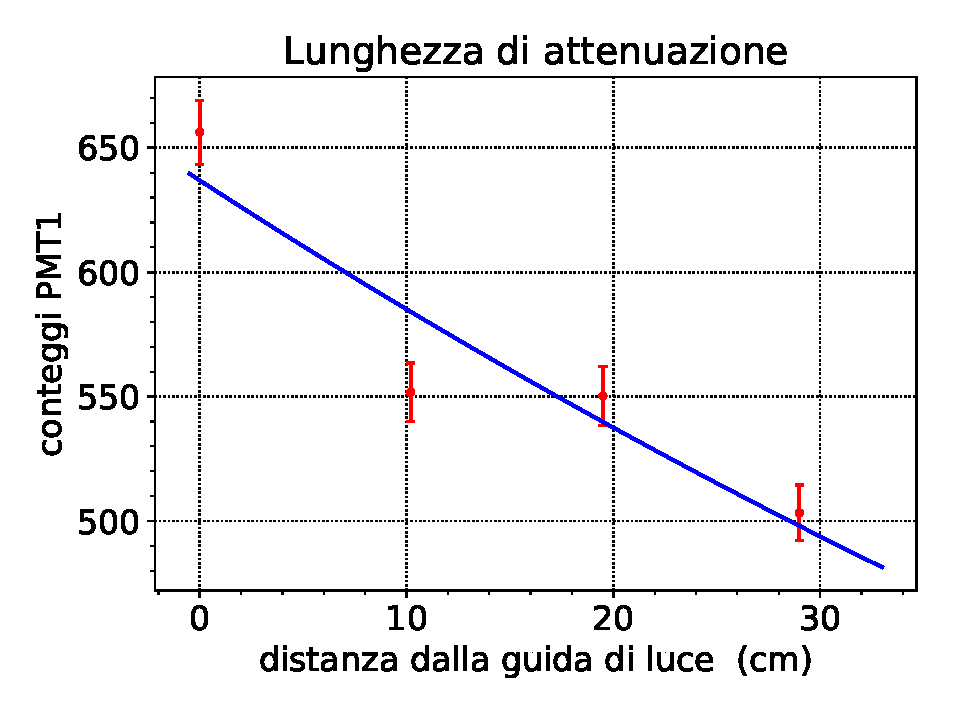
\includegraphics[width=8 cm]{atte}
\caption{Fit relativo alla lunghezza di attenuazione calcolata facendo la media per colonne.}
\label{atte}
\end{figure}

\begin{table}[h]
\centering
\begin{tabular}{| c | r @{$\pm$} l |}
\hline
colonna & \multicolumn{2}{c|}{media} \\
\hline
D & 503&11 \\
C & 550&12 \\
B & 551&12 \\
A & 656&13 \\
\hline
\end{tabular}
\caption{Dati del grafico in \autoref{atte}. La colonna D è quella più lontana dalla guida di luce.}
\end{table}

\subsubsection{Media per righe}

La seconda strategia adottata consiste nel fittare con la \eqref{exp} i conteggi di ogni riga separatamente e poi fare la media delle 4 lunghezze di attenuazione ottenute.
In \autoref{4atte} è possibile vedere le 4 curve con le relative funzioni di fit, mentre la \autoref{tab:righe} contiene i risultati del fit.

\begin{table}[h]
\centering
\begin{tabular}{| c | r @{$\pm$} l  | r @{$\pm$} l  | c |}
\hline
riga & \multicolumn{2}{c|}{$N_0$} & \multicolumn{2}{c|}{ $\lambda$ [\si{cm}] } & $\chi^2$ \\
\hline
1 & 711&19 & 121&23 & 1\\
2 & 638&32 & 127&47 & 4\\
3 & 632&60 & 73&30 & 15\\
4 & 565&21 & 228&111 & 2\\
\hline
\end{tabular}
\caption{Risultati restituiti dai fit presenti in \autoref{4atte} riga per riga. Tutti i fit hanno 2 gradi di libertà.}
\label{tab:righe}
\end{table}


La media dei parametri del fit restituisce $\langle\lambda\rangle=\SI{110\pm17}{cm}$ e $\langle N_0\rangle=643\pm13$.
\begin{figure}[h]
\centering
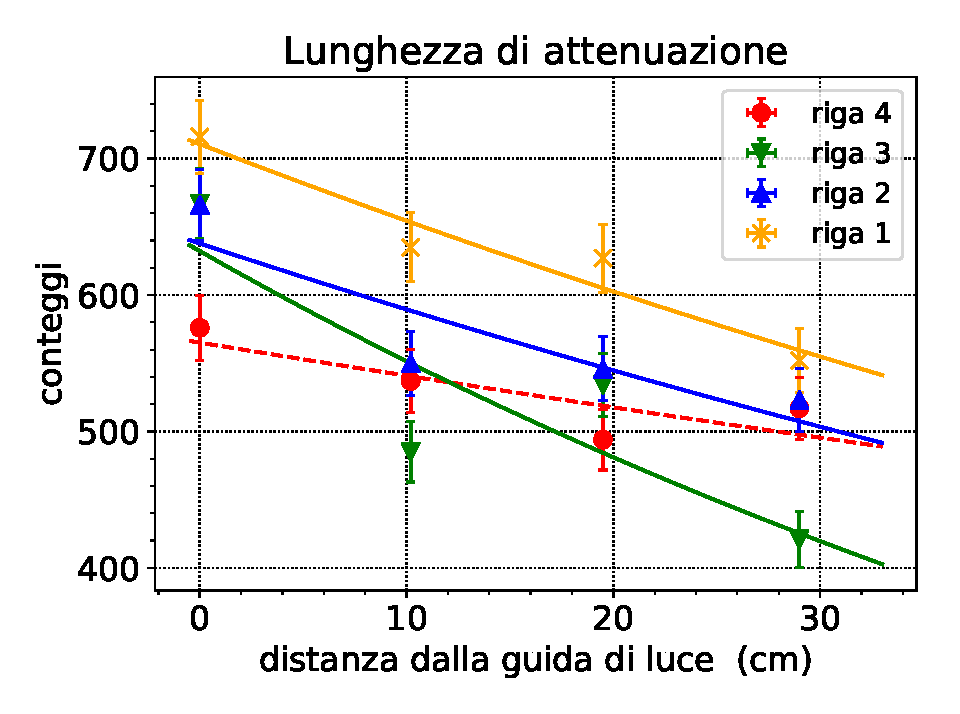
\includegraphics[width=8 cm]{4atte}
\caption{Fit relativo alla lunghezza di attenuazione calcolata facendo la media per righe. Il numero delle righe è quello indicato dalla figura \emph{autoref(schema)}.}
\label{4atte}
\end{figure}


\subsubsection{Limiti della misura}

I parametri ricavati dai 2 fit precedenti sono compatibili ed hanno un errore maggiore del 10\%. Con la strumentazione a nostra disposizione non è possibile determinare la lunghezza di attenuazione con maggiore precisione. Innanzitutto abbiamo usato un miniscint con un'area di \SI{14.7\pm0.9}{cm^2} la cui parte scintillante era appoggiata sul PM1 e la sua cassa \marginpar{``cassa'' va bene?} era appoggiata sulla struttura di metallo che lo circondava. L'angolo formato tra i due scintillatori per le misure periferiche è stato misurato e vale \SI{12.7\pm0.1}{\degree}, invece assume valori ogni volta diversi per le misure nelle altre caselle. Questo implica che l'area sottesa dal miniscint è maggiore di quella della sua parte scintillante e proprio per questo abbiamo deciso di non infittire la griglia disegnata sul PM1, considerando ogni casella di essa come l'area in cui si sarebbero misurate gran parte delle coincidenze. A questo effetto si aggiunge lo spessore del miniscint che vale all'incirca \SI{1}{cm} e può far scattare coincidenze anche quando un muone passa al di fuori della casella in cui il miniscint è stato posizionato. Questa evenienza diventa ancora più frequente quando il miniscint è inclinato perché, essendo in parte sollevato, permette ai muoni che lo hanno attraversato con angolo maggiore di giungere in un punto ancora più lontano della lastra sottostante. In questo caso lo spessore del miniscint può soltanto amplificarne l'effetto, in quanto se fosse inclinato con un angolo sufficientemente elevato riuscirebbe a intercettare sempre meglio  i muoni a grande angolo a discapito di quelli a piccolo angolo.
Le dimensioni trasversali del miniscint non permettono di definire la distanza dalla guida di luce meglio del loro valore e sappiamo anche che i fotoni, per arrivare al fotomoltiplicatore,  non percorrono una linea retta, ma vengono riflessi dal materiale che compone la lastra dello scintillatore e la guida di luce (riflessione totale) oppure dalla carta argentata che riveste gli stessi. Percorrendo queste traiettorie vengono attenuati ulteriormente e non abbiamo nessuna informazione su come essi arrivino al PMT1 né in linea di massima né caso per caso.

\subsubsection{Lunghezza di attenuazione in energia.}

Abbiamo analizzato i dati registrati dall'ADC collegata al PM1 (\autoref{fall}) facendo la media dei rilasci di energia per ogni colonna ma non abbiamo potuto estrarne alcuna informazione.
\marginpar{inventare una scusa}
\begin{figure}[h]
\centering
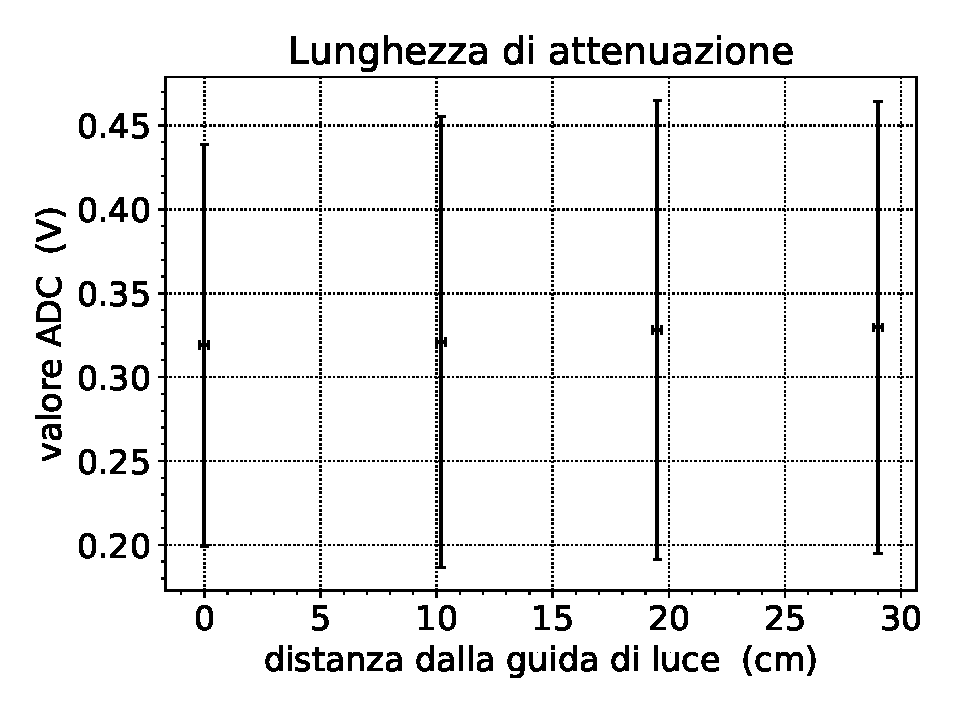
\includegraphics[width=8 cm]{fallimento}
\caption{Energia media giunta al pmt per ogni colonna.}
\label{fall}
\end{figure}

